% Input from the root of the supplied assignment2_writeup folder.
% Uses only graphicx, already loaded by the main report.
% Column-width figures can float nearby to avoid blank space at column breaks.
\section{Analysis 3: Does Cross-Option Variance Identify Answer Evidence?}
\label{sec:arun-analysis3}

\subsection{Motivation and Setup}
Idea~1 in our Project Proposal, \emph{Contrastive Evidence Selection}, asks whether we can choose useful video frames by comparing how well each frame matches the four possible answers. A frame may be related to the question without helping us choose an answer. We hypothesize that frames matching some answers more strongly than others provide better evidence for distinguishing between them. We test this idea without training a model, using a frozen Jina-CLIP-v2 encoder to compare images and text. The language analysis uses 280 questions from the portion of Video-MME reserved for exploring our methods rather than final testing. The visual analyses use 60 questions associated with 20 long videos from this same portion, covering different subject domains. We sample one frame per second. For each frame, we measure how closely it matches the question and each of the four question--answer pairs. To account for an answer that tends to match the entire video, we subtract that answer's average similarity across all frames from its score at each frame. We then measure how much these adjusted scores differ across the four answers. Larger differences give a higher variance score. Finally, we put question relevance and variance on comparable scales and average them with equal weight to obtain the combined selection score.

\subsection{Language and Cross-Modal Findings}
We encode each answer in two ways: as the answer text alone, and as ``Question: [question text] Answer: [answer text].'' We measure the average distance between the four resulting answer representations, where a larger distance means the encoder treats them as more different (Fig.~\ref{fig:arun-a3-language}). Including the question reduces this distance to 12--46\% of the answer-only value across task types. Counting answers are especially similar, suggesting that this encoding may struggle to distinguish numerical alternatives.

\begin{figure}[!htbp]
  \centering
  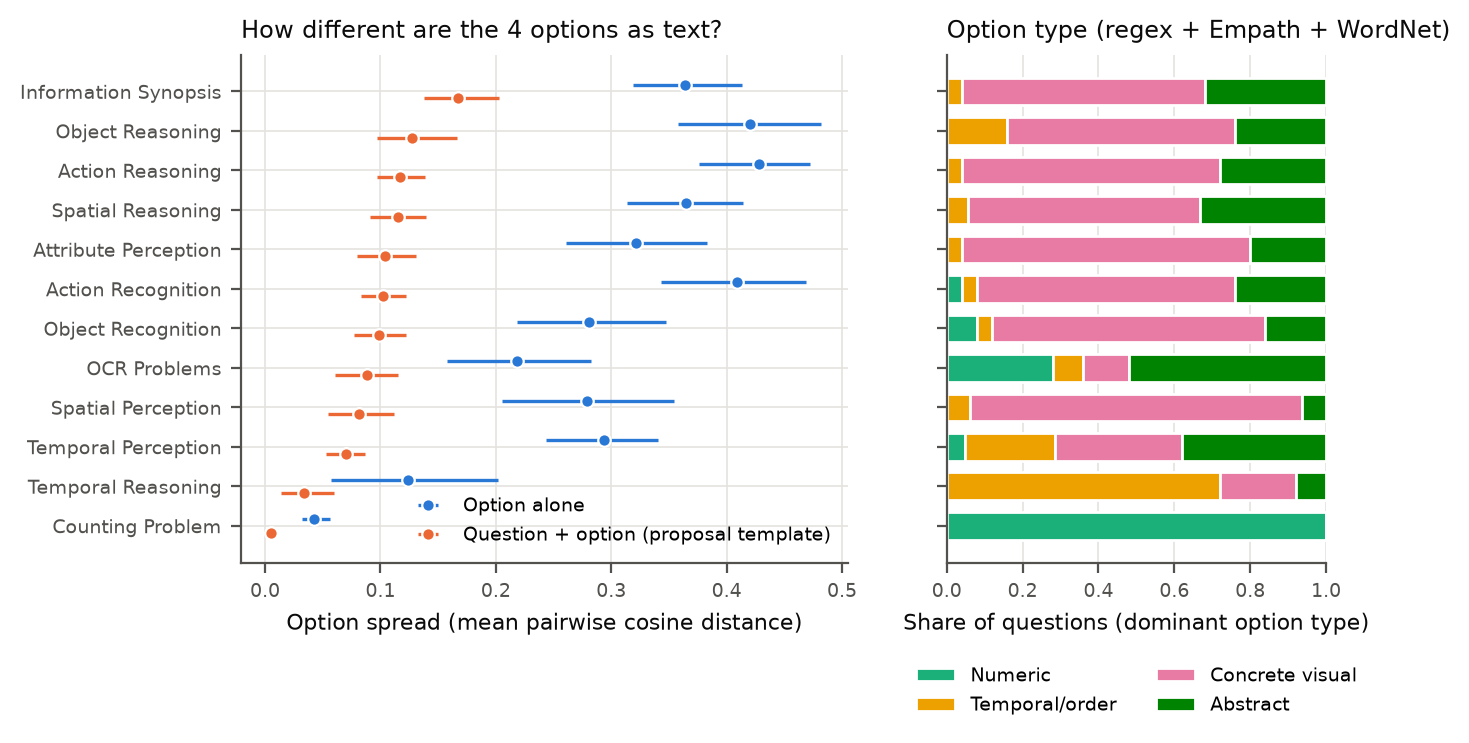
\includegraphics[width=\linewidth]{figures/fig1_option_spread.png}
  \caption{Option spread and dominant option types across 280 questions. Error bars: question-bootstrap 95\% intervals.}
  \label{fig:arun-a3-language}
\end{figure}

We then test whether variance reflects the video's content. For a given question, we score every frame against its four question--answer texts. We select the 16 frames with the largest differences among the adjusted answer scores and average their variance. We repeat this calculation on each of 19 other videos using the \emph{same} question--answer texts. These unrelated videos provide a baseline: does the question's own video separate its answers more strongly? The own-video average exceeds an approximate threshold based on this baseline for 36.7\% of questions and 57.1\% of perception questions (Fig.~\ref{fig:arun-a3-signal}). This suggests video-specific information, but does not establish that the selected frames support the correct answer.

\begin{figure}[!htbp]
  \centering
  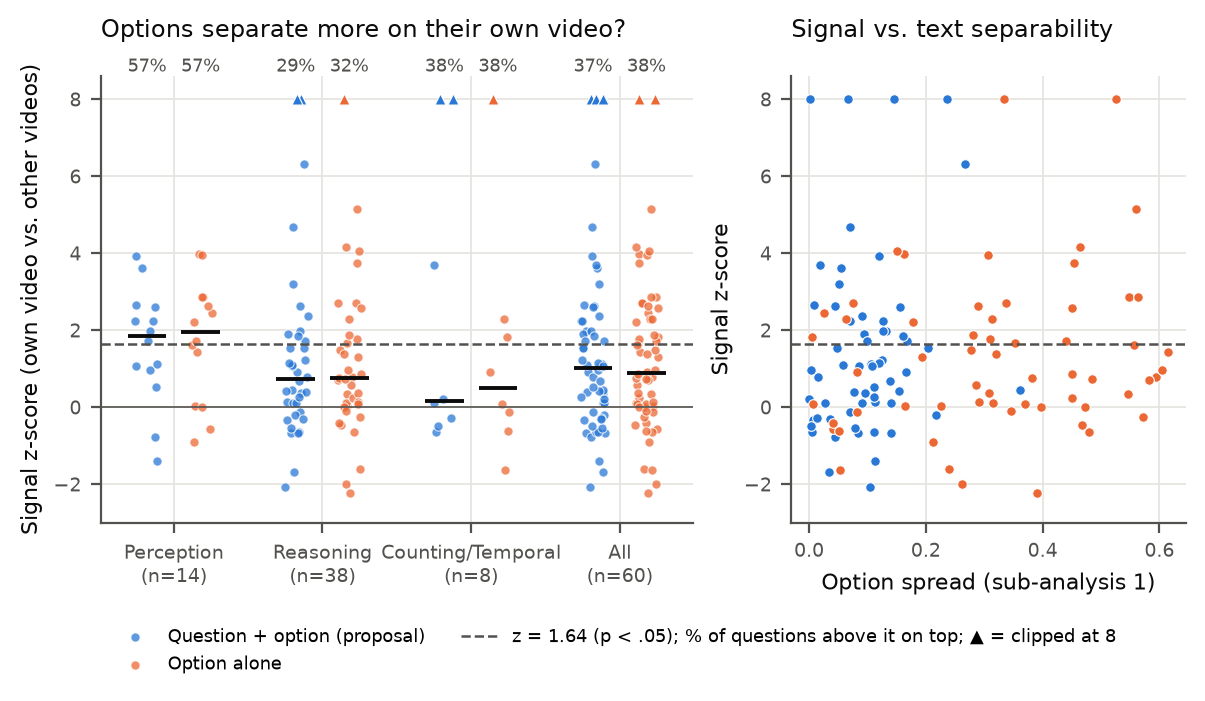
\includegraphics[width=\linewidth]{figures/fig2_signal_vs_null.png}
  \caption{Own-video variance versus 19 comparison videos. The $1.645$ threshold is a normal-reference diagnostic, not a calibrated $p$-value.}
  \label{fig:arun-a3-signal}
\end{figure}

\subsection{Evidence Selection Results}
We compare four ways to select 16 frames: evenly spaced sampling (uniform), question similarity (relevance), differences across answer scores (variance), and their combination (blend). Each frame votes for the answer with its highest adjusted similarity score. The answer receiving the most votes is the prediction, with ties resolved by adding the tied answers' scores across the selected frames. Accuracy is 31.7\% for uniform, 13.3\% for relevance, 20.0\% for variance, and 18.3\% for the blend (Fig.~\ref{fig:arun-a3-selection}). Using all frames gives 35.0\%. Variance therefore shows no accuracy improvement in this test. These votes use encoder scores, not a VLM reader.

\begin{figure}[!htbp]
  \centering
  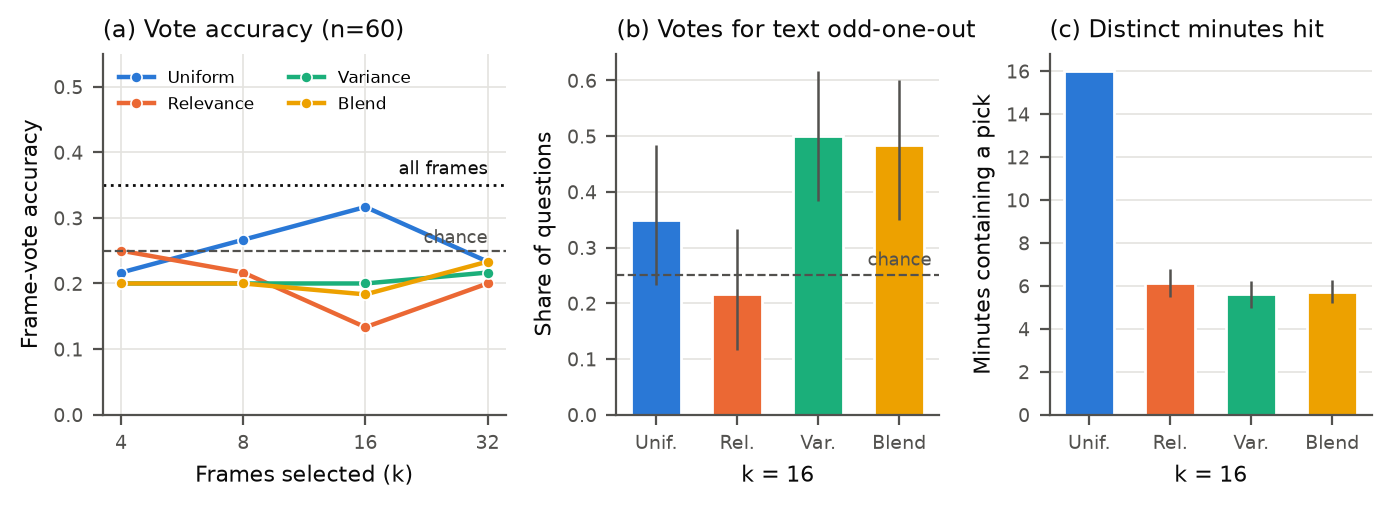
\includegraphics[width=\linewidth]{figures/fig3_frame_vote_opt_tmpl.png}
  \caption{Frame-vote accuracy, odd-one-out preference, and temporal coverage. Panels (b--c): $k=16$, with question-bootstrap 95\% intervals.}
  \label{fig:arun-a3-selection}
\end{figure}

Variance's final prediction is the answer whose text differs most from the other options in 50.0\% of questions, although that answer is correct in only 26.7\%. Both relevance and variance also cluster their selections: their 16 frames cover about six different minutes, compared with 16 for uniform sampling. In the profession example (Fig.~\ref{fig:arun-a3-example}), illustrated variance-selected frames favor the wrong answer, \emph{Police Officer}, while relevance-selected frames favor the correct \emph{Journalist}. Strong answer-score differences can therefore highlight a distractor rather than useful evidence.

\begin{figure}[!htbp]
  \centering
  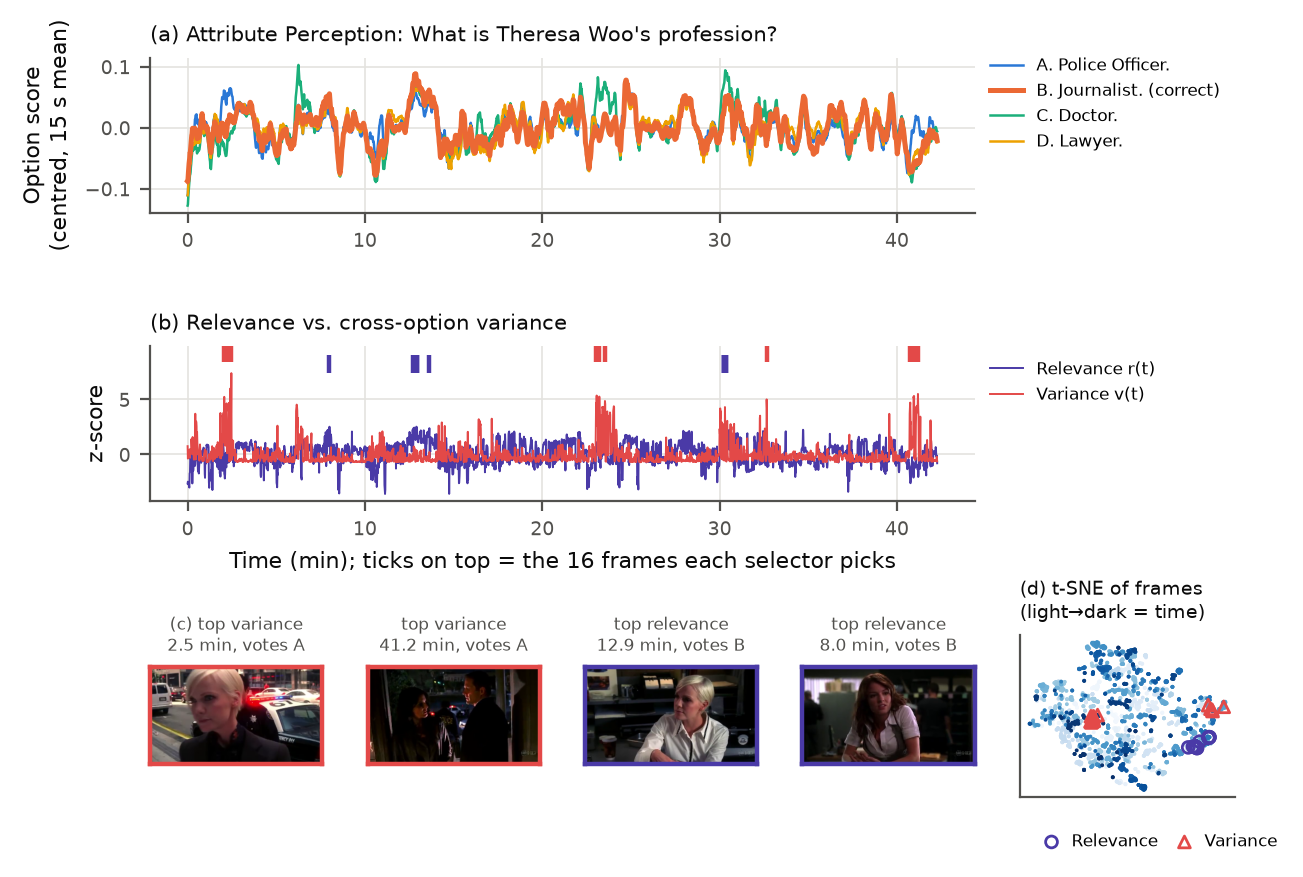
\includegraphics[width=\linewidth]{figures/fig4_example_opt_tmpl.png}
  \caption{Profession example: illustrated variance picks vote for \emph{Police Officer}. Relevance picks vote for the correct \emph{Journalist}. This example was selected for high signal.}
  \label{fig:arun-a3-example}
\end{figure}

\subsection{Discussion and Implications}
Our proposal assumed that larger differences across answer scores would help identify useful evidence. The analyses show that these differences can reflect video content, yet favor a wrong answer and concentrate selections in a few parts of the video. We therefore plan to revise how Idea~1 uses variance rather than assume it reliably identifies answer evidence.

First, we will compare encoding answers alone with encoding question--answer pairs, since shared question text reduces differences between answers. We will assess counting and ordering questions separately, where similar answer representations may make variance less useful. Second, we will spread selections across time to reduce clustering. Third, we will test selecting frames that match each possible answer, so one distinctive distractor cannot dominate the selection. These changes aim to give the reader broader evidence to compare. They remain untested. Because the current results use a small subset and encoder-based voting, we will evaluate the revised selectors with the same frozen Qwen2.5-VL reader and equal frame budgets, including uniform sampling as a baseline.
